\documentclass[a4paper,12pt]{article}

%%%%%%%%%%%%%%%%%%%
\usepackage[latin1]{inputenc} 		%Caracteres francais
\usepackage[T1]{fontenc} 		%Caracteres francais
\usepackage[francais]{babel}		%On ecrit en francais
\usepackage{geometry}
\usepackage{xcolor}
\usepackage{listings}
\usepackage[tikz]{bclogo}
\usepackage{hyperref}
\usepackage{amsmath}
\usepackage{nameref}

\hypersetup{colorlinks,citecolor=black,filecolor=black,linkcolor=red,urlcolor=blue}
\geometry{margin=2cm}
\title{Package ``fast-diagram.sty''}
\author{Raphaël ALLAIS}
\definecolor{fond}{RGB}{250,250,250}
\lstset{language=[LaTeX]TeX,columns=flexible,basicstyle=\ttfamily,texcsstyle=*\color{blue},identifierstyle=\color{brown},commentstyle=\color{gray}\itshape,
	moretexcs={FT,ST,fastDecalageTrait,FV,fastHauteurBoite,fastInterligne,fastLargeurBoite,fastEspaceColonne,fastReset,fastDecalageOuHorizontal,fastDecalageOuVertical,fastFT,fastST,fastVide,definecolor,fastSetCouleurBordures,fastSetCouleurTexte,fastSetCouleurFond}}
\newcommand{\cqd}{Ce qui donne :\\}
\newcommand{\comm}[1]{{\bfseries #1}}
\newcommand{\uem}	{\ensuremath{\footnotesize\text{ em}}}
\newcommand{\ucm}	{\ensuremath{\footnotesize\text{ cm}}}
\newcommand{\maref}[1]	{\nameref{#1} (p.\pageref{#1})}
\definecolor{couleurExemple}{RGB}{240,240,240}%{250,250,250} %Couleur du fond
\newenvironment{exemple}
		{\begin{bclogo}[couleur=couleurExemple,arrondi=0.3,noborder = true,logo=\bcloupe,epBarre = 0]{}}
		{\end{bclogo}\vspace{0.5cm}}

\lstnewenvironment{code}
		{\footnotesize\setbox1=\vbox
					\bgroup}
		{\egroup	
		\begin{center}
			\begin{minipage}{0.8\linewidth}
				\begin{bclogo}[couleur=white,logo=\bccrayon,noborder = true]{Code}
					\box1
				\end{bclogo}
			\end{minipage}
		\end{center}
}
%%%%%%%%%%%%%%%%%%%

\usepackage[raccourcis]{fast-diagram}

\begin{document}

	\maketitle


	\renewcommand{\fastLargeurBoite}{3.5cm}
	\renewcommand{\fastEspaceColonne}{5cm}
	\renewcommand{\fastEpaisseurTraits}{1.5pt}
	\renewcommand{\fastHauteurBoite}{2em}

	\section*{Table des matières}
	\vfill

	\begin{center}
		\footnotesize
		\begin{fast}{Package ``fast-diagram.sty''}
			\FT{\maref{intro}}{
				\FT{\maref{auteur}}{}
				\FT{\maref{rappel}}{}
				\FT{\maref{limitations}}{}
				}
			\FT{\maref{exemple}}{}
			\FT{\maref{MP}}{
				\FT{\maref{installation}}{}
				\FT{\maref{packages}}{}
				\FT{\maref{appel}}{}
				}
			\FT{\maref{commandes}}{
				\FT{\maref{environnement}}{}
				\FT{\maref{principe}}{}
				\FT{\maref{FT}}{}
				\FT{\maref{ST}}{}
				\FT{\maref{fvide}}{}
				\FT{\maref{trait}}{}
				}
			\FT{\maref{MIP}}{
				\FT{\maref{reset}}{}
				\FT{\maref{dimensions}}{}
				\FT{\maref{couleurs}}{}
				}
			\FT{\maref{tikzz}}{
				\FT{\maref{tikzpartout}}{}
				\FT{\maref{boites}}{}
				\FT{\maref{perso}}{}
				}
		\end{fast}
	\end{center}
	\vfill

	\fastReset

	\newpage

	\section{Introduction}\label{intro}
%=====================================

	\subsection{Le pourquoi du comment}\label{auteur}
	%--------------------------------

		En tant qu'enseignant en sciences industrielles pour l'ingénieur, j'ai réalisé ce package en vue de m'aider à rédiger mes cours.
		J'ai toutefois essayé de le rendre le plus paramétrable possible afin qu'il puisse être utilisé dans de nombreux cas.
		(d'autres options/paramètres peuvent éventuellement être rajoutés selon la demande...).

		Il s'agit de mon premier package \LaTeX.
		De plus, ce package fonctionne sur la bibliothèque \emph{TikZ}, que je connaissais jusqu'alors assez mal.
		Il n'est donc pas exclu qu'il y ait des bugs dans sa conception.
		Si vous voyez quelque chose d'anormal ou d'incohérent, ou si vous avez des remarques, n'hésitez pas à m'en faire part à l'adresse suivante :
		\href{mailto:allais.raphael@free.fr}{allais.raphael@free.fr}
		
		Pour le petite histoire, la difficulté pour réaliser ce package a été le caractère récursif du diagramme FAST.
		En effet, il semblerait que \emph{TikZ} gère très mal la portée locale des variables :
		Les variables d'une fonction \emph{enfant} écrasaient les variables de sa fonction \emph{parent}.
		Cela posait des problèmes sur l'alignement des boîtes.
		D'autre part, \emph{TikZ} propose déjà des diagrammes en arborescence, mais je n'ai pas su créer mes propres fonctions par dessus.

		Merci à Yannick Le Bras, Robert Papanicola et Xavier Pessoles pour leur aide et leurs conseils.


	\subsection{Petit rappel}\label{rappel}
	%-----------------------------
		Le diagramme ``\emph{\href{http://fr.wikipedia.org/wiki/Function_Analysis_System_Technique}{Function Analysis System Technique}}'', plus couramment appelé ``\emph{diagramme FAST}''
		est un outil de \textbf{\href{http://fr.wikipedia.org/wiki/Analyse_fonctionnelle_\%28conception\%29}{l'analyse fonctionnelle}},
		permettant de décrire et de décomposer hiérarchique une \emph{fonction de service} en sous-fonctions, appelées \emph{fonctions techniques}.
		L'aboutissement d'un tel schéma doit être un ensemble de choix concrets appelés ``\emph{solutions techniques}''.
		Historiquement, ce type de diagramme a été un passage indispensable dans le domaine de la conception et la rédaction des cahiers des charges.
		Aujourd'hui, une approche plus globale (mais partiellement basée sur des concepts similaires) est proposée au travers des diagrammes \href{http://fr.wikipedia.org/wiki/Systems_Modeling_Language}{SysML}.

		Pour plus de détail, n'hésitez pas à consulter les nombreux cours qui existent sur Internet.
		

	

	\subsection{Limitations - Perspectives}\label{limitations}
	%----------------------------------------

		Le package a été écrit pour répondre \textbf{aux principales attentes} du diagramme FAST.
		Il n'est cependant pas complet.
		Il n'est, par exemple, pas possible de relier \textbf{automatiquement} une solution technique commune à plusieurs fonctions techniques.
		Cette possibilité n'est toutefois pas exclue puisque les commandes de \emph{TikZ} sont autorisées à l'intérieur de l'environnement (voir \ref{tikzz}) et rien n'empêche de le faire ``\emph{à la main}''.
		N'hésitez donc pas à me faire part d'éventuelles autres fonctions à mettre en place.\newpage

	\section{Un exemple presque complet}\label{exemple}
%==========================================





	%%%%%%%%%%%%%%%%%%%%%%%%%%%%%%%%%%%%%%%%%%%%
	\begin{center}
	\footnotesize

	\definecolor{fastCouleurFondFS}{rgb}{0.90,0.85,0.70}
	\definecolor{fastCouleurFondFT}{rgb}{1,0.96,0.89}
	\definecolor{fastCouleurFondST}{rgb}{1,1,1}
	\renewcommand*{\fastHauteurBoite}{2.6em}
	\renewcommand*{\fastDecalageTrait}{-1.3em}
	\renewcommand*{\fastEspaceColonne}{9em}

	\begin{fast}{Déplacer la voiture téléguidée}
		\FT{Gérer les informations}
			{
			\FT{Démarrer la voiture}
				{
				\ST{Bouton marche/arrêt}
					[\FV{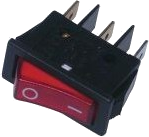
\includegraphics[height=1cm]{./sources_help/images/bouton.png}}]
				}
			\FT{Capter les ordres de la télécommande}
				{
				\ST{Antenne}
					[\FV{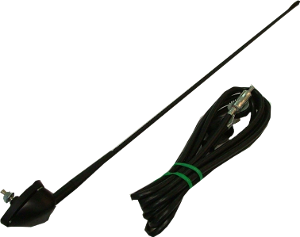
\includegraphics[height=1cm]{./sources_help/images/antenne.png}}]
				}
			\FT{Gérer les informations et distribuer}
				{
				\ST{Récepteur 2 voies}
					[\FV{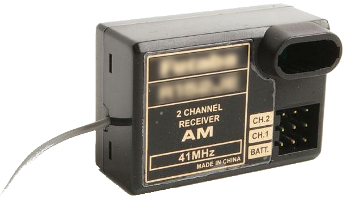
\includegraphics[height=1cm]{./sources_help/images/recepteur.png}}]
				}
			}
		\FT{Stocker l'énergie}
				{
				\trait{\ST{Batterie électrique}
					[\FV{
\includegraphics[height=1cm]{./sources_help/images/batterie.png}}]
				}}
		\FT{Propulser la voiture}
			{
			\FT{Transformer en énergie mécanique}
				{
				\ST{Moteur à courant continu}
					[\FV{
\includegraphics[height=1cm]{./sources_help/images/moteur.png}}]
				}
			\FT{Adapter l'énergie mécanique}
				{
				\ST{Engrenages}
					[\FV{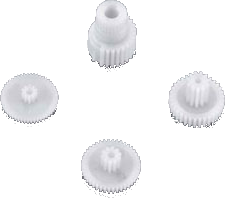
\includegraphics[height=1cm]{./sources_help/images/pignons.png}}]
				}
			\FT{Transmettre l'énergie mécanique}
				{
				\ST{Roues}
					[\FV{
\includegraphics[height=1cm]{./sources_help/images/roue.png}}]
				}
			}
		\FT{Diriger la voiture}
			{
			\FT{Transformer l'énergie}
				{
				\ST{Servomoteur}
					[\FV{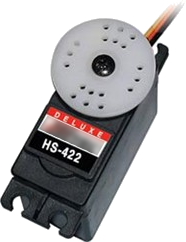
\includegraphics[height=1cm]{./sources_help/images/servomoteur.png}}]
				}
			\FT{Transmettre aux roues}
				{
				\ST{Biellettes}
					[\FV{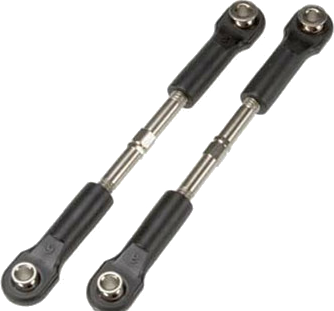
\includegraphics[height=1cm]{./sources_help/images/biellettes.png}}]
				}
			}
	\end{fast}
	\fastReset
	\end{center}
	%%%%%%%%%%%%%%%%%%%%%%%%%%%%%%%%%%%%%%%%%%%%


	L'exemple ci-dessus est donné par le code suivant :

%######################################
\begin{lstlisting}
\begin{center}
\footnotesize

\definecolor{fastCouleurFondFS}{rgb}{0.90,0.85,0.70}
\definecolor{fastCouleurFondFT}{rgb}{1,0.96,0.89}
\definecolor{fastCouleurFondST}{rgb}{1,1,1}
\renewcommand*{\fastHauteurBoite}{2.6em}
\renewcommand*{\fastDecalageTrait}{-1.3em}
\renewcommand*{\fastEspaceColonne}{9em}

\begin{fast}{Déplacer la voiture téléguidée}
	\FT{Gérer les informations}
		{\FT{Démarrer la voiture}
			{\ST{Bouton marche/arrêt}
				[\FV{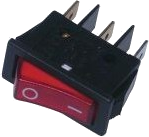
\includegraphics[height=1cm]
				{./sources_help/images/bouton.png}}]
			}
		\FT{Capter les ordres de la télécommande}
			{\ST{Antenne}
				[\FV{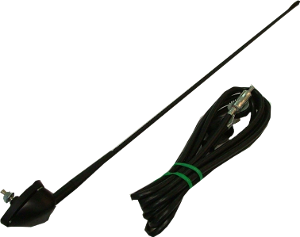
\includegraphics[height=1cm]
				{./sources_help/images/antenne.png}}]
			}
		\FT{Gérer les informations et distribuer}
			{\ST{Récepteur 2 voies}
				[\FV{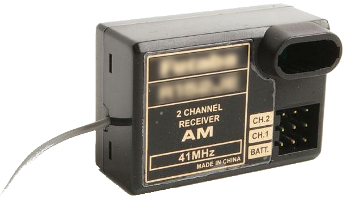
\includegraphics[height=1cm]
				{./sources_help/images/recepteur.png}}]
		}	}
	\FT{Stocker énergie}
		{\trait{
			\ST{Batterie électrique}
				[\FV{
\includegraphics[height=1cm]
				{./sources_help/images/batterie.png}}]
		}	}
	\FT{Propulser la voiture}
		{\FT{Transformer en énergie mécanique}
			{\ST{Moteur à courant continu}
				[\FV{
\includegraphics[height=1cm]
				{./sources_help/images/moteur.png}}]
			}
		\FT{Adapter l'énergie mécanique}
			{\ST{Engrenages}
				[\FV{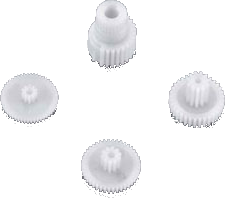
\includegraphics[height=1cm]
				{./sources_help/images/pignons.png}}]
			}
		\FT{Transmettre l'énergie mécanique}
			{\ST{Roues}
				[\FV{
\includegraphics[height=1cm]
				{./sources_help/images/roue.png}}]
		}	}
	\FT{Diriger la voiture}
		{\FT{Transformer l'énergie}
			{\ST{Servomoteur}
				[\FV{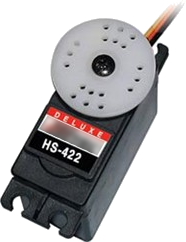
\includegraphics[height=1cm]
				{./sources_help/images/servomoteur.png}}]
			}
		\FT{Transmettre aux roues}
			{\ST{Biellettes}
				[\FV{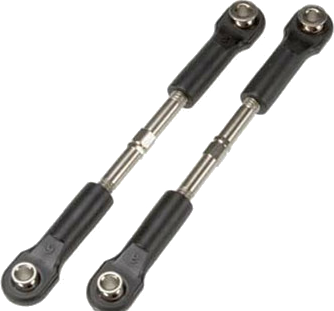
\includegraphics[height=1cm]
				{./sources_help/images/biellettes.png}}]
		}	}
\end{fast}
\fastReset
\end{center}
\end{lstlisting}
	
\newpage

	\section{Mise en place du package}\label{MP}
%==================================


	\subsection{Installation}\label{installation}
	%--------------------------

		Le package s'installe comme n'importe quel autre.
		Après l'avoir téléchargé, copier le :
		\begin{itemize}
			\item soit dans le dossier du document que vous êtes en train de rédiger (c'est une méthode facile, mais il ne sera valable que pour ce document-là)
			\item soit dans un des dossiers par défaut de latex.
				L'emplacement de ces dossiers dépendent du logiciel et du système d'exploitation utilisé (Windows, Mac, Linux, etc.).
		\end{itemize}

	\subsection{Packages requis}\label{packages}
	%-----------------------------------

		Pour que le package fonctionne, vous devez déjà avoir les packages suivants d'installés :
		\begin{itemize}
			\item \href{http://sourceforge.net/projects/pgf/}{\textbf{TikZ}} : Package de dessin vectoriel sur lequel repose le diagramme fast,
			\item \href{http://www.ctan.org/pkg/ifthen}{\textbf{ifthen}} : Package permettant une compilation à choix multiple,
			\item \href{http://www.ctan.org/pkg/relsize}{\textbf{relsize}} : Package permettant de gérer les longueurs relatives (em, ...)
			\item \href{http://tug.ctan.org/tex-archive/macros/latex/contrib/xargs}{\textbf{xarg}} : Package permettant de créer des commandes à plusieurs arguments optionnels.
		\end{itemize}

	\subsection{Appel du package ``fast-diagram.sty''}\label{appel}
	%-------------------------------

		L'appel du package se fait simplement en écrivant dans l'entête du document :
%#########################
\begin{code}
\usepackage{fast-diagram}
\end{code}
%########################
		Afin d'éviter d'éventuels conflits entre packages, toutes les commandes utilisées ici sont précédées du préfixe {\color{blue}\verb'fast'}
		(par exemple {\color{blue}\verb'\fastFT'} pour désigner la fonction technique \verb'FT').
		Pour la mise en place de raccourcis, l'option {\color{blue}\verb'[raccourcis]'} peut être apportée dans le package de la manière suivante :
%#########################
\begin{code}
\usepackage[raccourcis]{fast-diagram}
\end{code}
%########################
		Les raccourcis seront développés plus tard.\newpage

	\section{D�tail des commandes}\label{commandes}
%=====================================


	\subsection{Environement ``fast''}\label{environnement}
	%------------------------------------

		Le diagramme fast est plac� dans l'environnement {\color{blue}\verb'\begin{fast}...\end{fast}'}.
		Cet environnement prend comme argument la \emph{fonction de service} que l'on souhaite d�velopper.

\begin{code}%##################################################################
\begin{fast}{Fonction de Service}
	%Votre diagramme FAST
\end{fast}
\end{code}%##################################################################
		\cqd
%%%%%%%%%%%%%%%%%%%%%%%%%%%%%%%%%%%%%%%%%%%%%%%%%%%%%%%%%%%%%
\begin{exemple}
\begin{fast}{Fonction de Service}
	%Votre diagramme FAST
\end{fast}
\end{exemple}
%%%%%%%%%%%%%%%%%%%%%%%%%%%%%%%%%%%%%%%%%%%%%%%%%%%%%%%%%%%%%

		A l'int�rieur de l'environnement \verb!fast!, on va alors venir placer chacune des fonctions techniques, solutions techniques, etc.
		Ces commandes vont �tre d�crites dans les paragraphes suivants.





	\subsection{Principe des commandes}\label{principe}
	%----------------------------------------------

		Une fois l'environnement fast ouvert, le but du jeu va �tre de cr�er des fonctions (c'est � dire des ``\emph{boites}'') � l'int�rieur, reli�es entre elles de mani�re hi�rarchique.

		Il existe plusieurs ``boites'' diff�rentes qui seront chacune d�velopp�es dans les paragraphes suivants.

		Chaque boite poss�de un ``\textbf{parent}'' en amont, un ``\textbf{texte}'' � l'int�rieur et �ventuellement une ou plusieurs ``\textbf{descendances}'' en aval.

		\begin{center}
			\begin{fast}{Parent}
				\definecolor{fastCouleurFondFT}{rgb}{1,0.5,0.5}
				\FT{texte}{\fastReset
					\FT{Descendance 1}{}
					\FT{Descendance 2}{}
					}
			\end{fast}
		\end{center}
		

		Le texte de chaque fonction est pass� en premier argument de la commande.

		On parlera de fonctions ``\emph{s\oe urs}'' lorsque ces fonctions sont en parall�les, issues d'un m�me parent.
		Les commandes permettant de cr�er plusieurs fonctions s\oe urs sont plac�es les unes � la suite des autres.

%##################################################################
\begin{code}
\begin{fast}{PARENT}
	\une_fonction{texte}{Descendance de la fonction}
	\une_fonction_soeur{texte}{Descendance de la fonction soeur}
\end{fast}
\end{code}
%##################################################################

		On parlera de fonctions ``\emph{filles}'' les fonctions descendant d'un parent.
		Les fonctions filles sont pass�es en deuxi�me argument de leur parent.

%##################################################################
\begin{code}
\begin{fast}{PARENT}
	\une_fonction{texte}{
				\une_fonction_fille{texte}{descendance}
				\une_autre_fonction_fille{texte}{descendance}
			}
\end{fast}
\end{code}
%##################################################################

	En pratique, la descendance peut �tre n'importe quelle fonction \emph{TikZ} (voir \ref{tikzz}).
	Elle peut �galement ne rien comporter.

	La suite de ce chapitre va pr�senter les diff�rentes fonctions disponibles.




	\subsection{Fonction technique}\label{FT}
	%----------------------------------------------

		{\color{blue}\verb'\fastFT'} (raccourci : {\color{blue}\verb'\FT'}) est une commande ``de base'' du diagramme FAST.
		Elle s'emploie de la mani�re suivante :

%##################################################################
\begin{code}
\begin{fast}{Fonction de Service}
	\fastFT{Fonction technique FT}
		{
			%Descendance
		}
\end{fast}
\end{code}
%##################################################################
		\cqd
%%%%%%%%%%%%%%%%%%%%%%%%%%%%%%%%%%%%%%%%%%%%%%%%%%%%%%%%%%
\begin{exemple}
\begin{fast}{Fonction de Service}
	\fastFT{Fonction technique FT}
		{
			%Descendance
		}
\end{fast}
\end{exemple}
%%%%%%%%%%%%%%%%%%%%%%%%%%%%%%%%%%%%%%%%%%%%%%%%%%%%%%%%%%

		Voici un exemple d'utilisation en s�rie et en parall�le :

%##################################################################
\begin{code}
\begin{fast}{Fonction de Service}
	\fastFT{FT1}
		{
			\fastFT{FT11}{}
			\fastFT{FT12}{}
		}
	\fastFT{FT2}
		{
			\fastFT{FT21}{}
			\fastFT{FT22}{}
		}
\end{fast}
\end{code}
%##################################################################
		\cqd
%%%%%%%%%%%%%%%%%%%%%%%%%%%%%%%%%%%%%%%%%%%%%%%%%%%%%%%%%%
\begin{exemple}
\begin{fast}{Fonction de Service}
	\fastFT{FT1}
		{
			\fastFT{FT11}{}
			\fastFT{FT12}{}
		}
	\fastFT{FT2}
		{
			\fastFT{FT21}{}
			\fastFT{FT22}{}
		}
\end{fast}
\end{exemple}
%%%%%%%%%%%%%%%%%%%%%%%%%%%%%%%%%%%%%%%%%%%%%%%%%%%%%%%%%%

		Si le premier argument est vide, cela revient � faire un trait horizontal, au m�me titre que que la fonction {\color{blue}\verb'\fastFTrait'} (voir \ref{trait}).

		La commande {\color{blue}\verb'\fastFT'} peut �galement prendre un mot-cl� en options :
		%\begin{itemize}
			%\item le mot cl� {\color{blue}\verb'[tempo]'} permet de rajouter un connecteur entre la fonction courante et la fonction situ�e au dessus (Ne fonctionne pas si la fonction est vide).
			 le mot cl� {\color{blue}\verb'[ou]'} ; il d�cale l�g�rement le connecteur pour repr�senter un liaison ``\emph{ou}'' (voir la mise en forme au paragraphe \ref{dimensions}).
		%\end{itemize}

%##################################################################
\begin{code}
\begin{fast}{FS}
	\FT{FT1}
		{
			\fastFT{FT1}{}
			\fastFT[ou]{FT2}{}
		}
\end{fast}
\end{code}
%##################################################################
		\cqd
%%%%%%%%%%%%%%%%%%%%%%%%%%%%%%%%%%%%%%%%%%%%%%%%%%%%%%%%%%
\begin{exemple}
\begin{fast}{FS}
	\fastFT{FT1}{}
	\fastFT[ou]{FT2}{}
\end{fast}
\end{exemple}
%%%%%%%%%%%%%%%%%%%%%%%%%%%%%%%%%%%%%%%%%%%%%%%%%%%%%%%%%%



	\subsection{Solution technique }\label{ST}
	%----------------------------------------------

		{\color{blue}\verb'\fastST'} (raccourci : {\color{blue}\verb'\ST'}) prend un seul argument : le contenu de la solution technique.

%##################################################################
\begin{code}
\begin{fast}{Fonction de Service}
	\fastST{Solution technique}
\end{fast}
\end{code}
%##################################################################
		\cqd
%%%%%%%%%%%%%%%%%%%%%%%%%%%%%%%%%%%%%%%%%%%%%%%%%%%%%%%%%%
\begin{exemple}
\begin{fast}{Fonction de Service}
	\fastST{Solution technique}
\end{fast}
\end{exemple}
%%%%%%%%%%%%%%%%%%%%%%%%%%%%%%%%%%%%%%%%%%%%%%%%%%%%%%%%%%

		Normalement, la solution technique correspond � la fin d'une branche du diagramme FAST.
		C'est pourquoi elle ne requi�re pas d'autre argument.
		Toutefois, pour des besoins sp�cifiques (commentaire, image, etc.), on peut lui rajouter une descendance en option :

%##################################################################
\begin{code}
\begin{fast}{Fonction de Service}
	\fastST{Solution technique}[\fastVide{Commentaire...}]
\end{fast}
\end{code}
%##################################################################
		\cqd
%%%%%%%%%%%%%%%%%%%%%%%%%%%%%%%%%%%%%%%%%%%%%%%%%%%%%%%%%%
\begin{exemple}
\begin{fast}{Fonction de Service}
	\fastST{Solution technique}[\fastVide{Commentaire...}{}]
\end{fast}
\end{exemple}
%%%%%%%%%%%%%%%%%%%%%%%%%%%%%%%%%%%%%%%%%%%%%%%%%%%%%%%%%%


	\subsection{Fonction vide}\label{fvide}
	%-----------------------------------------

		{\color{blue}\verb'\fastVide'} (raccourci : {\color{blue}\verb'\FV'}) permet de faire une case sans connecteur ni bordure.

%####################################
\begin{code}
\begin{fast}{Fonction de Service}
	\fastFT{FT1}	{
				\fastVide{Boite sans trait}
				\fastVide{Autre boite sans trait}
		}
	\fastFT{FT2}{		\fastVide{Encore une boite sans trait}}
\end{fast}
\end{code}
%####################################
		\cqd
%%%%%%%%%%%%%%%%%%%%%%%%%%%%%%%%%%%%%%%%%%%%%%%%%%%%%%%%%%
\begin{exemple}
\begin{fast}{Fonction de Service}
	\fastFT{FT1}	{
				\fastVide{Boite sans trait}
				\fastVide{Autre boite sans trait}
		}
	\fastFT{FT2}{		\fastVide{Encore une boite sans trait}}
\end{fast}
\end{exemple}
%%%%%%%%%%%%%%%%%%%%%%%%%%%%%%%%%%%%%%%%%%%%%%%%%%%%%%%%%%

		Tout comme pour la boite ``solution technique'', cette fonction est destin�e � �tre en bout de branche du diagramme.
		On ne demande donc pas de descendance.
		Toutefois, on peut la lui proposer en argument optionnel :

%##################################################################
\begin{code}
\begin{fast}{Fonction de Service}
	\fastVide{Boite vide}[\fastFT{Descendance}{}]
\end{fast}
\end{code}
%##################################################################
\cqd
%%%%%%%%%%%%%%%%%%%%%%%%%%%%%%%%%%%%%%%%%%%%%%%%%%%%%%%%%%
\begin{exemple}
\begin{fast}{Fonction de Service}
	\fastVide{Boite vide}[\fastFT{Descendance}{}]
\end{fast}
\end{exemple}
%%%%%%%%%%%%%%%%%%%%%%%%%%%%%%%%%%%%%%%%%%%%%%%%%%%%%%%%%%


	\subsection{Trait continu}\label{trait}
	%-----------------------------------------

		{\color{blue}\verb'\fastTrait'} (raccourci : {\color{blue}\verb'\trait'}) repr�sente un simple trait.
		Il permet en effet de tracer un connecteur directement de la colonne $(n-1)$ � $(n+1)$, en ``sautant'' la colonne $(n)$.
		Le seul argument demand� est la descendance de ce connecteur.
		La fonction technique {\color{blue}\verb'\fastFT'} avec un premier argument vide r�alise la m�me chose.

%##################################################################
\begin{code}
\begin{fast}{Fonction de Service}
	\fastFT{De base}{}
	\fastTrait	{
		\fastFT{avec fastTrait}{}
		}
	\fastFT{}	{
		\fastFT{avec fastFT dont le $1^{er}$ argument est vide}{}
		}
\end{fast}
\end{code}
%##################################################################
		\cqd
%%%%%%%%%%%%%%%%%%%%%%%%%%%%%%%%%%%%%%%%%%%%%%%%%%%%%%%%%%
\begin{exemple}
\begin{fast}{Fonction de Service}
	\fastFT{De base}{}
	\fastTrait	{
		\fastFT{avec fastTrait}{}
		}
	\fastFT{}	{
		\fastFT{avec fastFT dont le $1^{er}$ argument est vide}{}
		}
\end{fast}
\end{exemple}
%%%%%%%%%%%%%%%%%%%%%%%%%%%%%%%%%%%%%%%%%%%%%%%%%%%%%%%%%%



\newpage

	\section{Mise en forme}\label{MIP}
%========================

	\subsection{Reset}\label{reset}
	%--------------------------

		{\color{blue}\verb'\fastReset'} permet de remettre les paramètres par défaut.



	\subsection{Les dimensions}\label{dimensions}
	%-------------------------------

		Les dimensions du diagramme sont réglées via plusieurs commandes.
		En voici la liste :
		\begin{itemize}
			\item {\color{blue}\verb'\fastInterligne'} : espace entre le bas de la boite la plus grande de la ligne en cours, et le haut des boites de la ligne suivante.
									Ce nombre doit être positif.
									(Par défaut : $0.5\uem$)
			\item {\color{blue}\verb'\fastLargeurBoite'} : largeur des boites (Par défaut : $7\uem$)
			\item {\color{blue}\verb'\fastHauteurBoite'} : hauteur \textbf{minimum} des boites (Par défaut : $0$)
			\item {\color{blue}\verb'\fastEspaceColonne'} :  distance entre le coin supérieur gauche d'une boite et le coin supérieur gauche de sa voisine.
									(Par défaut : $10\uem$)
			\item {\color{blue}\verb'\fastDecalageTrait'} : permet de décaler le connecteur par rapport au haut de la boite.
									(Par défaut : $-0.6\uem$)
			\item {\color{blue}\verb'\fastEpaisseurTraits'} : épaisseur des traits (bordures et connecteurs). (Par défaut : $0.05\uem$)
			\item {\color{blue}\verb'\fastDecalageOuVertical'} : Décalage vertical du connecteur ``OU''. (Par défaut : $0.4\uem$)
			\item {\color{blue}\verb'\fastDecalageOuHorizontal'} :	Décalage horizontal du connecteur ``OU''. (Par défaut : $-0.4\uem$)
		\end{itemize}

		Les deux dernières fonctions peuvent être utiles si plusieurs connecteur ``OU'' sont utilisés sur la même lignée.

		Toutes ces commandes peuvent être redéfinies via la fonction la fonction {\color{blue}\verb'\renewcommand'} (ou {\color{blue}\verb'\renewcommand*'}).
		Voici ci-dessous une série d'exemples illustrant chacune de ces fonctions.


		\subsubsection{Exemple : interlignes}\label{interligne}
		%-----------------------------------

%#####################################################
\begin{code}
\begin{fast}{Avant}	%Interligne par défaut
	\fastFT{FT1}{
		\fastFT{FT11 avec un peu de texte}{
			\fastFT{FT111}{}}}
	\fastFT{FT2}{
		\fastFT{FT21}{
			\fastFT{FT211}{}}}
\end{fast}

\renewcommand*{\fastInterligne}{1cm}	%Nouvel interligne
\begin{fast}{Après}
	\fastFT{FT1}{
		\fastFT{FT11 avec un peu de texte}{
			\fastFT{FT111}{}}}
	\fastFT{FT2}{
		\fastFT{FT21}{
			\fastFT{FT211}{}}}
\end{fast}
\fastReset	%Remise à zéro
\end{code}
%#####################################################
		\cqd
%%%%%%%%%%%%%%%%%%%%%%%%%%%%%%%%%%%%%%%%%%%%%%%%%%%%%%%%
\begin{exemple}
\begin{fast}{Avant}	%Interligne par défaut
	\fastFT{FT1}{
		\fastFT{FT11 avec un peu de texte}{
			\fastFT{FT111}{}}}
	\fastFT{FT2}{
		\fastFT{FT21}{
			\fastFT{FT211}{}}}
\end{fast}
\renewcommand*{\fastInterligne}{1cm}	%Nouvel interligne
\begin{fast}{Après}
	\fastFT{FT1}{
		\fastFT{FT11 avec un peu de texte}{
			\fastFT{FT111}{}}}
	\fastFT{FT2}{
		\fastFT{FT21}{
			\fastFT{FT211}{}}}
\end{fast}
\fastReset	%Remise à zéro
\end{exemple}
%%%%%%%%%%%%%%%%%%%%%%%%%%%%%%%%%%%%%%%%%%%%%%%%%%%%%%%%



		\subsubsection{Exemple : largeur des boîtes}\label{largeur}
		%-----------------------------------


%###############################################
\begin{code}
\begin{fast}{Avant}
	\fastFT{FT1}{}
	\fastFT{FT2}{}
\end{fast}

\renewcommand*{\fastLargeurBoite}{1.5cm}	%Nouvelle largeur de boite
\begin{fast}{Après}
	\fastFT{FT1}{}
	\fastFT{FT2}{}
\end{fast}
\fastReset
\end{code}
%###############################################
\cqd
%%%%%%%%%%%%%%%%%%%%%%%%%%%%%%%%%%%%%%%%%%%%%%%%%%%%%%%%
\begin{exemple}
\begin{fast}{Avant}
	\fastFT{FT1}{}
	\fastFT{FT2}{}
\end{fast}
\renewcommand*{\fastLargeurBoite}{1.5cm}
\begin{fast}{Après}
	\fastFT{FT1}{}
	\fastFT{FT2}{}
\end{fast}
\fastReset
\end{exemple}
%%%%%%%%%%%%%%%%%%%%%%%%%%%%%%%%%%%%%%%%%%%%%%%%%%%%%%%%



		\subsubsection{Exemple : hauteur des boîtes}\label{hauteur}
		%-----------------------------------


%###############################################
\begin{code}
\begin{fast}{Avant}
	\fastFT{FT1}{	\FT{FT11}{}
			\FT{FT12 FT12 FT12 FT12}{}}
	\fastFT{FT2}{	\FT{FT21}{}
			\FT{FT22}{}}
\end{fast}
\renewcommand*{\fastHauteurBoite}{3em}
\begin{fast}{Après}
	\fastFT{FT1}{	\FT{FT11}{}
			\FT{FT12 FT12 FT12 FT12}{}}
	\fastFT{FT2}{	\FT{FT21}{}
			\FT{FT22}{}}
\end{fast}
\fastReset
\end{code}
%###############################################
\cqd
%%%%%%%%%%%%%%%%%%%%%%%%%%%%%%%%%%%%%%%%%%%%%%%%%%%%%%%%
\begin{exemple}
\begin{fast}{Avant}
	\fastFT{FT1}{	\FT{FT11}{}
			\FT{FT12 FT12 FT12 FT12}{}}
	\fastFT{FT2}{	\FT{FT21}{}
			\FT{FT22}{}}
\end{fast}
\renewcommand*{\fastHauteurBoite}{3em}
\begin{fast}{Après}
	\fastFT{FT1}{	\FT{FT11}{}
			\FT{FT12 FT12 FT12 FT12}{}}
	\fastFT{FT2}{	\FT{FT21}{}
			\FT{FT22}{}}
\end{fast}
\fastReset
\end{exemple}
%%%%%%%%%%%%%%%%%%%%%%%%%%%%%%%%%%%%%%%%%%%%%%%%%%%%%%%%


		\subsubsection{Exemple : espace entre colonnes}\label{espace}
		%-----------------------------------


%###############################################
\begin{code}
\begin{fast}{Avant}
	\fastFT{FT1}{
		\fastFT{FT11}{}}
	\fastFT{FT2}{
		\fastFT{FT21}{}}
\end{fast}

\renewcommand*{\fastEspaceColonne}{6cm}	%Nouvel espace inter-colonnes
\begin{fast}{Après}
	\fastFT{FT1}{
		\fastFT{FT11}{}}
	\fastFT{FT2}{
		\fastFT{FT21}{}}
\end{fast}
\fastReset
\end{code}
%###############################################
\cqd
%%%%%%%%%%%%%%%%%%%%%%%%%%%%%%%%%%%%%%%%%%%%%%%%%%%%%%%%
\begin{exemple}
\begin{fast}{Avant}
	\fastFT{FT1}{
		\fastFT{FT11}{}}
	\fastFT{FT2}{
		\fastFT{FT21}{}}
\end{fast}
\renewcommand*{\fastEspaceColonne}{6cm}
\begin{fast}{Après}
	\fastFT{FT1}{
		\fastFT{FT11}{}}
	\fastFT{FT2}{
		\fastFT{FT21}{}}
\end{fast}
\fastReset
\end{exemple}
%%%%%%%%%%%%%%%%%%%%%%%%%%%%%%%%%%%%%%%%%%%%%%%%%%%%%%%%





	\subsubsection{Exemple : décalage des connecteurs}\label{decalage}
	%----------------------------------------

%###############################################
\begin{code}
\begin{fast}{Avant}
	\fastFT{FT1}{}
	\fastFT{FT2}{}
\end{fast}

\renewcommand*{\fastDecalageTrait}{-13pt}	%Nouveau décalage des connecteur
\begin{fast}{Après}
	\fastFT{FT1}{}
	\fastFT{FT2}{}
\end{fast}
\fastReset
\end{code}
%###############################################
\cqd
%%%%%%%%%%%%%%%%%%%%%%%%%%%%%%%%%%%%%%%%%%%%%%%%%%%%%%%%
\begin{exemple}
\begin{fast}{Avant}
	\fastFT{FT1}{}
	\fastFT{FT2}{}
\end{fast}
\renewcommand*{\fastDecalageTrait}{-13pt}
\begin{fast}{Après}
	\fastFT{FT1}{}
	\fastFT{FT2}{}
\end{fast}
\fastReset
\end{exemple}
%%%%%%%%%%%%%%%%%%%%%%%%%%%%%%%%%%%%%%%%%%%%%%%%%%%%%%%%







	\subsubsection{Exemple : épaisseur des traits}\label{epaisseur}
	%----------------------------------


%###############################################
\begin{code}
\begin{fast}{Avant}
	\fastFT{FT1}{}
	\fastFT{FT2}{}
\end{fast}

\renewcommand*{\fastEpaisseurTraits}{2pt}	%Nouvelle épaisseur de traits
\begin{fast}{Après}
	\fastFT{FT1}{}
	\fastFT{FT2}{}
\end{fast}
\fastReset
\end{code}
%###############################################
\cqd
%%%%%%%%%%%%%%%%%%%%%%%%%%%%%%%%%%%%%%%%%%%%%%%%%%%%%%%%
\begin{exemple}
\begin{fast}{Avant}
	\fastFT{FT1}{}
	\fastFT{FT2}{}
\end{fast}
\renewcommand*{\fastEpaisseurTraits}{2pt}
\begin{fast}{Après}
	\fastFT{FT1}{}
	\fastFT{FT2}{}
\end{fast}
\fastReset
\end{exemple}
%%%%%%%%%%%%%%%%%%%%%%%%%%%%%%%%%%%%%%%%%%%%%%%%%%%%%%%%



	\subsubsection{Exemple : Décalage des connecteur ``OU''}\label{connecteursOU}
	%----------------------------------


%###############################################
\begin{code}
\begin{fast}{Avant}
	\fastFT{FT1}{}
	\fastFT{FT2}{}
	\fastFT[ou]{FT3}{}
	\fastFT[ou]{FT4}{}
\end{fast}

\renewcommand*{\fastDecalageOuVertical}{3pt}	%Redécalage vertical...
\renewcommand*{\fastDecalageOuHorizontal}{-3pt}	%... et horizontal du 1er "OU"
\begin{fast}{Après}
	\fastFT{FT1}{}
	\fastFT{FT2}{}
	\fastFT[ou]{FT3}{}
	\renewcommand{\fastDecalageOuVertical}{6pt}	%Décalage vertical...
	\renewcommand{\fastDecalageOuHorizontal}{-6pt}	%...et horizontal...
	\fastFT[ou]{FT4}{}				% ...du 2eme "OU"
\end{fast}
\fastReset
\end{code}
%###############################################
\cqd
%%%%%%%%%%%%%%%%%%%%%%%%%%%%%%%%%%%%%%%%%%%%%%%%%%%%%%%%
\begin{exemple}
\begin{fast}{Avant}
	\fastFT{FT1}{}
	\fastFT{FT2}{}
	\fastFT[ou]{FT3}{}
	\fastFT[ou]{FT4}{}
\end{fast}
\renewcommand*{\fastDecalageOuVertical}{3pt}
\renewcommand*{\fastDecalageOuHorizontal}{-3pt}
\begin{fast}{Après}
	\fastFT{FT1}{}
	\fastFT{FT2}{}
	\fastFT[ou]{FT3}{}
	\renewcommand{\fastDecalageOuVertical}{6pt}
	\renewcommand{\fastDecalageOuHorizontal}{-6pt}
	\fastFT[ou]{FT4}{}
\end{fast}
\fastReset
\end{exemple}
%%%%%%%%%%%%%%%%%%%%%%%%%%%%%%%%%%%%%%%%%%%%%%%%%%%%%%%%







	\subsection{Couleurs}\label{couleurs}
	%--------------------------

		Il est possible de modifier les couleurs de plusieurs éléments tels que :
		\begin{itemize}
			\item \textbf{la fonction de service} (la première case),
			\item \textbf{les fonctions techniques},
			\item \textbf{les solutions techniques},
			\item \textbf{les boîtes vides},
			\item \textbf{les connecteurs}.
		\end{itemize}
		Pour chacun des quatre premiers points précédents, on peut définir :
		\begin{itemize}
			\item la couleur du \textbf{texte},
			\item la couleur du \textbf{fond} (sauf boite vide),
			\item la couleur du \textbf{cadre} (sauf boite vide).
		\end{itemize}
		Tout cela donne un total de $11$ couleurs, définies par les noms suivants :
		\begin{itemize}
			\item {\color{blue}\verb'fastCouleurTexteFS'} : Couleur du texte de la fonction de service (la $1^{ere}$ boite),
			\item {\color{blue}\verb'fastCouleurBorduresFS'} : Couleur de bordure de la fonction de service (la $1^{ere}$ boite),
			\item {\color{blue}\verb'fastCouleurFondFS'} : Couleur du fond de la fonction de service (la $1^{ere}$ boite),
			\item {\color{blue}\verb'fastCouleurTexteFT'} : Couleur du texte des fonctions techniques,
			\item {\color{blue}\verb'fastCouleurBorduresFT'} : Couleur de bordure des fonctions techniques,
			\item {\color{blue}\verb'fastCouleurFondFT'} : Couleur du fond des fonctions techniques,
			\item {\color{blue}\verb'fastCouleurTexteST'} : Couleur du texte des solutions techniques,
			\item {\color{blue}\verb'fastCouleurBorduresST'} : Couleur de bordure des solutions techniques,
			\item {\color{blue}\verb'fastCouleurFondST'} : Couleur du fond des solutions techniques,
			\item {\color{blue}\verb'fastCouleurTexteFV'} : Couleur du texte de la fonction de boite vide,
			\item {\color{blue}\verb'fastCouleurConnecteurs'} : Couleur des connecteurs.
		\end{itemize}

		Toutes ces couleurs peuvent être redéfinies par la fonction {\color{blue}\verb'\definecolor'}
		(voir le package \href{http://www.ctan.org/tex-archive/macros/latex/contrib/xcolor/}{xcolor}) :

%###################################################
\begin{code}
\definecolor{fastCouleurTexteFS}	{named}	{white}
\definecolor{fastCouleurBorduresFS}	{named}	{red}
\definecolor{fastCouleurFondFS}		{named}	{red}

\definecolor{fastCouleurTexteFT}	{rgb}	{1,0,1}
\definecolor{fastCouleurBorduresFT}	{rgb}	{0,1,0}
\definecolor{fastCouleurFondFT}		{rgb}	{1,1,0}

\definecolor{fastCouleurTexteST}	{named}	{brown}
\definecolor{fastCouleurBorduresST}	{named}	{blue}
\definecolor{fastCouleurFondST}		{rgb}	{0.5,1,1}

\definecolor{fastCouleurConnecteurs}	{rgb}	{1,0.5,1}
\begin{fast}{FS1}
	\fastFT{FT1}{
		\fastST{Sol 1}}
	\fastFT{}{
		\fastST{Sol2}}
\end{fast}
\fastReset
\end{code}
%###################################################
\cqd
%%%%%%%%%%%%%%%%%%%%%%%%%%%%%%%%%%%%%%%%%%%%%%%%%%%%%%%%
\begin{exemple}
\definecolor{fastCouleurTexteFS}	{named}	{white}
\definecolor{fastCouleurBorduresFS}	{named}	{red}
\definecolor{fastCouleurFondFS}		{named}	{red}

\definecolor{fastCouleurTexteFT}	{rgb}	{1,0,1}
\definecolor{fastCouleurBorduresFT}	{rgb}	{0,1,0}
\definecolor{fastCouleurFondFT}		{rgb}	{1,1,0}

\definecolor{fastCouleurTexteST}	{named}	{brown}
\definecolor{fastCouleurBorduresST}	{named}	{blue}
\definecolor{fastCouleurFondST}		{rgb}	{0.5,1,1}

\definecolor{fastCouleurConnecteurs}	{rgb}	{1,0.5,1}
\begin{fast}{FS1}
	\fastFT{FT1}{
		\fastST{Sol 1}}
	\fastFT{}{
		\fastST{Sol2}}
\end{fast}
\fastReset
\end{exemple}
%%%%%%%%%%%%%%%%%%%%%%%%%%%%%%%%%%%%%%%%%%%%%%%%%%%%%%%%

	Pour aller plus vite, trois commandes servent de raccourci :
	\begin{itemize}
		\item {\color{blue}\verb'\fastSetCouleurBordures[type]{couleur}'} : permet de changer la couleur de toutes les bordures,
		\item {\color{blue}\verb'\fastSetCouleurTexte[type]{couleur}'} : permet de changer la couleur de tout le texte,
		\item {\color{blue}\verb'\fastSetCouleurTraits[type]{couleur}'} : permet de changer la couleur de toutes les lignes (bordures + connecteurs),
		\item {\color{blue}\verb'\fastSetCouleurFond[type]{couleur}'} : permet de changer la couleur du fond de toutes les boites,
	\end{itemize}
	où {\color{blue}\verb'[type]'} est le type d'affectation (\emph{rgb},\emph{cmyk},\emph{named}(par défaut),...)
	et {\color{blue}\verb'[couleur]'} est la couleur, relativement à {\color{blue}\verb'[type]'} (voir {\color{blue}\verb'\definecolor'} du package \href{http://www.ctan.org/tex-archive/macros/latex/contrib/xcolor/}{xcolor}).


%###################################################
\begin{code}
\fastSetCouleurBordures{red}
\fastSetCouleurTexte[rgb]{1,1,1}
\fastSetCouleurFond{black}
\begin{fast}{FS1}
	\fastFT{FT1}{
		\fastST{Sol 1}}
	\fastFT{}{
		\fastST{Sol2}}
\end{fast}
\fastReset
\end{code}
%###################################################
\cqd
%%%%%%%%%%%%%%%%%%%%%%%%%%%%%%%%%%%%%%%%%%%%%%%%%%%%%%%%
\begin{exemple}
\fastSetCouleurBordures{red}
\fastSetCouleurTexte[rgb]{1,1,1}
\fastSetCouleurFond{black}
\begin{fast}{FS1}
	\fastFT{FT1}{
		\fastST{Sol 1}}
	\fastFT{}{
		\fastST{Sol2}}
\end{fast}
\fastReset
\end{exemple}
%%%%%%%%%%%%%%%%%%%%%%%%%%%%%%%%%%%%%%%%%%%%%%%%%%%%%%%%


\newpage

	\section{Jouons avec TikZ\label{tikzz}}
%=======================================



	\subsection{TikZ dans le diagramme FAST}\label{tikzpartout}
	%------------------------------------------------

		L'environnement FAST est un environnement \emph{TikZ}.
		Il est donc possible d'y ajouter n'importe quelle fonction de dessin de \emph{TikZ}.
		Il en est de m�me pour les descendances des fonctions.
%##########################################
\begin{code}
\begin{fast}{Fonction de Service}
	\FT{FT1}{\draw [shift={(4,-1)},rotate=45,scale=0.5,ball color=blue]
		(0,0) .. controls +(0,2) and +(0,3) .. (3,0)
		.. controls +(0,-2) and +(0,2) .. (0,-4)
		.. controls +(0,2) and +(0,-2) .. (-3,0)
		.. controls +(0,2) and +(0,2) .. (0,0);
		}		%Exemple pris dans ``TikZ pour l'impatient''
	\FT{FT2}{}
\end{fast}
\end{code}
%##########################################
		\cqd
%%%%%%%%%%%%%%%%%%%%%%%%%%%%%%%%%%%%%%%%%%
\begin{exemple}
\begin{fast}{Fonction de Service}
	\FT{FT1}{\draw [shift={(4,-1)},rotate=45,scale=0.5,ball color=blue]
			(0,0) .. controls +(0,2) and +(0,3) .. (3,0)
			.. controls +(0,-2) and +(0,2) .. (0,-4)
			.. controls +(0,2) and +(0,-2) .. (-3,0)
			.. controls +(0,2) and +(0,2) .. (0,0);}
			%Exemple pris dans ``TikZ pour l'impatient''
	\FT{FT2}{}
\end{fast}
\end{exemple}
%%%%%%%%%%%%%%%%%%%%%%%%%%%%%%%%%%%%%%%%%%

		Il est � noter que dans l'exemple pr�c�dent, la seconde ligne du diagramme ne tient pas compte de la ``place'' que prend notre dessin.
		Pour que ce soit le cas, il faut que la descendance (c'est � dire le dessin) ``marque'' sa place en cr�ant une coordonn�e correspondant au point le plus bas du dessin.
		C'est sur ce point que la seconde ligne va se baser.

		Ce point doit �tre enregistr� dans la variable {\color{blue}\verb'BoiteMinimums'} de la mani�re suivante :
%##########################################
\begin{code}
\coordinate (BoiteMinimums) at (X,Y);
\end{code}
%##########################################
		o� le couple $(X, Y)$ est la coordonn�es du minimum.

		Par exemple :
%##########################################
\begin{code}
\begin{fast}{Fonction de Service}
	\FT{FT1}{\draw [shift={(4,-1)},rotate=45,scale=0.5,ball color=blue]
		(0,0) .. controls +(0,2) and +(0,3) .. (3,0)
		.. controls +(0,-2) and +(0,2) .. (0,-4)
		.. controls +(0,2) and +(0,-2) .. (-3,0)
		.. controls +(0,2) and +(0,2) .. (0,0);
		\coordinate (BoiteMinimums) at (0,-2.5);
		}	%Exemple pris dans ``TikZ pour l'impatient''
	\FT{FT2}{}
\end{fast}
\end{code}
%##########################################
		\cqd
%%%%%%%%%%%%%%%%%%%%%%%%%%%%%%%%%%%%%%%%%%
\begin{exemple}
\begin{fast}{Fonction de Service}
	\FT{FT1}{\draw [shift={(4,-1)},rotate=45,scale=0.5,ball color=blue]
		(0,0) .. controls +(0,2) and +(0,3) .. (3,0)
		.. controls +(0,-2) and +(0,2) .. (0,-4)
		.. controls +(0,2) and +(0,-2) .. (-3,0)
		.. controls +(0,2) and +(0,2) .. (0,0);
		\coordinate (BoiteMinimums) at (0,-2.5);}
		%Exemple pris dans ``TikZ pour l'impatient''
	\FT{FT2}{}
\end{fast}
\end{exemple}
%%%%%%%%%%%%%%%%%%%%%%%%%%%%%%%%%%%%%%%%%%

	\subsection{Gestion des bo�tes}\label{boites}
	%-----------------------------------------

	Les boites cr��es dans le diagramme FAST sont r�alis�es par la fonction {\color{blue}\verb'\node'} de \emph{TikZ}.
	Ces bo�tes sont nomm�es sous la forme suivante : {\color{blue}\verb'\fastBoiteX'} o� {\color{blue}\verb'X'} est remplac� par le num�ro de la boite.
	Ce num�ro est d�fini par ordre de cr�ation des boites : de gauche � droite, de haut en bas.
	Voici un exemple faisant appara�tre le nom des boites :
	\begin{center}
		\begin{fast}{fastBoite0}
			\FT{fastBoite1}{\FT{fastBoite2}{}
					\FT{fastBoite3}{\FT{fastBoite4}{}}}
			\FT{fastBoite5}{\FT{fastBoite6}{}
					\FT{fastBoite7}{}}
		\end{fast}
	\end{center}

	Partant de l�, il est alors possible de r�aliser des modifications manuelles sur le diagramme.
	Par exemple, pour avoir une solution technique commune � deux fonctions techniques :
%##########################################
\begin{code}
\begin{fast}{Fonction de service}
	\fastFT{FT1}{\fastST{ST}}
	\fastFT{FT2}{}
	\draw[line width=\fastEpaisseurTraits]
		(fastBoite3.east) -| ($0.5*(fastBoite2.north west)
		+0.5*(fastBoite1.north east)+(0,\fastDecalageTrait)$);
\end{fast}
\end{code}
%##########################################
	\cqd
%%%%%%%%%%%%%%%%%%%%%%%%%%%%%%%%%%%%%%%%%%
\begin{exemple}
\begin{fast}{Fonction de service}
	\fastFT{FT1}{\fastST{ST}}
	\fastFT{FT2}{}
	\draw[line width=\fastEpaisseurTraits](fastBoite3.east)	-| ($0.5*(fastBoite2.north west)+0.5*(fastBoite1.north east)+(0,\fastDecalageTrait)$);
\end{fast}
\end{exemple}
%%%%%%%%%%%%%%%%%%%%%%%%%%%%%%%%%%%%%%%%%%

	\subsection{Cr�er sa propre boite}\label{perso}
	%--------------------------------------

	Les boites sont � peu pr�s toutes cr��es sur le m�me mod�le et il est possible d'en cr�er d'autres :
%##########################################
\begin{code}
\newcommand*{\maBoite}[2]{
	\fastAvanceColonne		%On avance d'une colonne
	\addtocounter{cptBoite}{1}	%On incremente le numero de la boite
	%%%%%%%%%%%%%%%%%%%%%%%
	%Cr�er votre boite ici :
	\node [anchor=north west] (noeud \thecptAbscisse) at
		($(\posX,0)+(BoiteMinimums)$) {#1};
	%%%%%%%%%%%%%%%%%%%%%%
	\node[inner sep=0,fit=(noeud \thecptAbscisse.north west)
		(noeud \thecptAbscisse.south east)]
		(fastBoite\thecptBoite) {};%Boite de nommage
	\fastTraceConnecteurs
	%%%%%%%%%%%%%%%%%%%%%%%%%
	%Votre descendance :
	#2
	%%%%%%%%%%%%%%%%%%%%%%%%%
	\fastEnregistreMinimum		%Enregistre le minimum de la boite
	\fastReculeColonne		%Recule d'une colonne
}
\end{code}
%##########################################


	Le n\oe ud cr�� sous la ligne ``{\color{blue}\verb'Cr�er votre boite ici'}'' est la boite que vous allez afficher.
	C'est elle que vous allez pouvoir modifier pour l'adapter � vos besoins.
	Ce n\oe ud doit obligatoirement porter le nom {\color{blue}\verb'(noeud \thecptAbscisse)'}.
	Les autres commandes ne doivent pas �tre chang�es.

	Voici un exemple :
%##########################################
\begin{code}
  \newcommand*{\maBoite}[2]{
	\fastAvanceColonne		%On avance d'une colonne
	\addtocounter{cptBoite}{1}	%On incremente le numero de la boite
	%%%%%%%%%%%%%%%%%%%%%%%
	%Cr�er votre boite ici
	\node [anchor=north west,draw,rounded corners=3pt,
		aspect=2.5,text=red](noeud \thecptAbscisse)
		at ($(\posX,0)+(BoiteMinimums)$) {#1};
	%%%%%%%%%%%%%%%%%%%%%%
	\node[inner sep=0,fit=(noeud \thecptAbscisse.north west)
		(noeud \thecptAbscisse.south east)]
		(fastBoite\thecptBoite) {};
	\fastTraceConnecteurs
	%%%%%%%%%%%%%%%%%%%%%%%%%
	%Votre descendance
	#2
	%%%%%%%%%%%%%%%%%%%%%%%%%
	\fastEnregistreMinimum		%Enregistre le minimum de la boite
	\fastReculeColonne		%Recule d'une colonne
}

\begin{fast}{Fonction de Service}
	\maBoite{Ma boite}
		{\fastST{Solution}}
	\FT{Fonction}{\maBoite{Ma boite bis}{}
			\fastFT{Fonction}{}}
\end{fast}
\end{code}
%##########################################
\cqd
%%%%%%%%%%%%%%%%%%%%%%%%%%%%%%%%%%%%%%%%%%
\begin{exemple}
  \newcommand*{\maBoite}[2]{
	\fastAvanceColonne		%On avance d'une colonne
	\addtocounter{cptBoite}{1}	%On incremente le numero de la boite
	%%%%%%%%%%%%%%%%%%%%%%%
	%Cr�er votre boite ici
	\node [anchor=north west,draw,rounded corners=3pt,aspect=2.5,text=red](noeud \thecptAbscisse) at ($(\posX,0)+(BoiteMinimums)$) {#1};
	%%%%%%%%%%%%%%%%%%%%%%
	\node[inner sep=0,fit=(noeud \thecptAbscisse.north west)
		(noeud \thecptAbscisse.south east)]
		(fastBoite\thecptBoite) {};%Boite vide par dessus, aux bonne dimension, afin de lui donner un nom
	\fastTraceConnecteurs
	%%%%%%%%%%%%%%%%%%%%%%%%%
	%Votre descendance
	#2
	%%%%%%%%%%%%%%%%%%%%%%%%%
	\fastEnregistreMinimum		%Enregistre le minimum de la boite
	\fastReculeColonne		%Recule d'une colonne
}

\begin{fast}{Fonction de Service}
	\maBoite{Ma boite}
		{\fastST{Solution}}
	\FT{Fonction}{\maBoite{Ma boite bis}{}
			\fastFT{Fonction}{}}
\end{fast}
\end{exemple}
%%%%%%%%%%%%%%%%%%%%%%%%%%%%%%%%%%%%%%%%%%\newpage

\end{document}